%-------------------------------------------------------------------------------
% Copyright (c) 2015-2016 University of Luxembourg.
% All rights reserved. This program and the accompanying materials
% are made available under the terms of the Eclipse Public License v1.0
% which accompanies this distribution, and is available at
% http://www.eclipse.org/legal/epl-v10.html
% 
% Contributors:
%     Alfredo Capozucca - initial API and implementation
%     Benoit Ries - minor updates
%     Nicolas Guelfi - most content from messirbook
%-------------------------------------------------------------------------------
%%%%%%%%%%%%%%%%%%%%%%%%%%%%%%%%%%%%%%%%%%%%%%%%%%
\PassOptionsToPackage{usenames,svgnames,table}{xcolor}
\documentclass[graybox,envcountchap,sectrefs]{./../lu.uni.lassy.excalibur.standard.report.libraries/styles/svmono}  
%%%%%%%%%%%%%%%%%%%%%%%%%%%%%%%%%%%%%%%%%%%%%%%%%% 
%%% DO NOT CHANGE THE ORDER
\usepackage{./../lu.uni.lassy.excalibur.standard.report.libraries/styles/style-messir-common}
\usepackage{./../lu.uni.lassy.excalibur.standard.report.libraries/styles/style-messir-report-post}
\usepackage{breakurl} 
\usepackage{graphicx}
\graphicspath{ {images/} }
%--------------------------------------------
  
% DOCUMENT BEGIN
%--------------------------------------------
\begin{document}
%-------------------------------------------------------------------------------
 
\newgeometry{textwidth=17cm,textheight=23.7cm} 
 
\definecolor{lightgray}{RGB}{201,201,201}
\definecolor{lightred}{RGB}{250,112,97}
\definecolor{lightgreen}{RGB}{179,250,140}

\definecolor{msrtextcl}{RGB}{0,0,0}
\definecolor{msrkeycl}{RGB}{127,0,85}
\definecolor{msrcmtcl}{RGB}{201,201,201}
\definecolor{keywordcolor}{RGB}{30,144,255}

\definecolor{aqua_blue}{RGB}{0,139,145}
\definecolor{dark_green}{RGB}{0,128,0}
\definecolor{dark_blue}{RGB}{45,45,138}

\definecolor{msrcolor01}{rgb}{0.96,0.59,0.48}
\definecolor{msrcolor02}{rgb}{1.00,0.97,0.60}
\definecolor{msrcolor03}{rgb}{0.51,0.79,0.61}
\definecolor{msrcolor04}{rgb}{0.43,0.81,0.96}
\definecolor{msrcolor05}{rgb}{0.52,0.58,0.79}
\definecolor{msrcolor06}{rgb}{0.96,0.61,0.76}
\definecolor{msrcolor07}{rgb}{0.98,0.68,0.51}
\definecolor{msrcolor08}{rgb}{0.77,0.88,0.61}
\definecolor{msrcolor09}{rgb}{0.49,0.66,0.85}
\definecolor{msrcolor10}{rgb}{0.96,0.60,0.62}
\definecolor{msrcolor11}{rgb}{0.64,0.83,0.61}
\definecolor{msrcolor12}{rgb}{0.63,0.53,0.75}
\definecolor{msrcolor13}{rgb}{0.99,0.78,0.54}
\definecolor{msrcolor14}{rgb}{0.53,0.51,0.74}
\definecolor{msrcolor15}{rgb}{0.48,0.80,0.79}
\definecolor{msrcolor16}{rgb}{0.74,0.55,0.75}
\definecolor{msrcolor17}{rgb}{0.90,0.79,0.08}
\definecolor{msrcolor18}{rgb}{1.00,1.00,0.00}
\definecolor{msrcolor19}{rgb}{1.00,0.00,0.50}

\definecolor{sepcolor000000}{rgb}{0, 0, 0}
\definecolor{sepcolor101010}{rgb}{0.10, 0.10, 0.10}
\definecolor{sepcolor202020}{rgb}{0.20, 0.20, 0.20}
\definecolor{sepcolor303030}{rgb}{0.30, 0.30, 0.30}
\definecolor{sepcolor404040}{rgb}{0.10, 0.10, 0.10}
\definecolor{sepcolor505050}{rgb}{0,1,.5}
\definecolor{sepcolor907908}{rgb}{0,1,.5}

\definecolor{sepregioncolor01}{rgb}{0.00,0.66,0.00}
\definecolor{sepregioncolor02}{rgb}{1.00,1.00,0.00}
\definecolor{sepregioncolor03}{rgb}{1.00,0.97,0.60}
\definecolor{sepregioncolor04}{rgb}{0.64,0.83,0.61}
\definecolor{sepregioncolor05}{rgb}{0.95,0.36,0.00}
\definecolor{sepregioncolor06}{rgb}{0.90,0.79,0.08}
\definecolor{sepregioncolor07}{rgb}{0.63,0.53,0.75}
\definecolor{sepregioncolor08}{rgb}{0.99,0.78,0.54}
\definecolor{sepregioncolor09}{rgb}{0.96,0.61,0.76}
\definecolor{sepregioncolor10}{rgb}{1.00,0.00,0.50}

\colorlet{msrcolorbrown}{red!40!black!80}


% Messir General
%----------------------------------------------------------

% quotePosition + quoteWidth + quotefillColor + quoteElement + quotedElement + allImageScale
\newcommand{\msrcallouted}[6]{
\scalebox{#1}{\parbox{\linewidth}{
  \begin{tikzpicture}
      \node [rectangle callout,callout relative pointer={#4},text width=#5,fill=#6,rounded corners] (tmpcall) at (0,0) {#3};
      \node at (tmpcall.pointer){#2};
  \end{tikzpicture}
}}
}

% Vresion wihtout scaling the quoted text
\pgfkeys{%
    /calloutquote/.cd,
    width/.code                   =  {\def\calloutquotewidth{#1}},
    position/.code                =  {\def\calloutquotepos{#1}}, 
    author/.code                  =  {\def\calloutquoteauthor{#1}},
    /calloutquote/.unknown/.code   =  {\let\searchname=\pgfkeyscurrentname
                                 \pgfkeysalso{\searchname/.try=#1,
    /tikz/\searchname/.retry=#1},\pgfkeysalso{\searchname/.try=#1,
                                  /pgf/\searchname/.retry=#1}}
                            }  

\newcommand\calloutquote[2][]{%
  \pgfqkeys{/calloutquote}{#1}
  \node [rectangle callout,callout relative pointer={\calloutquotepos},text width=\calloutquotewidth,/calloutquote/.cd,#1] (tmpcall) at (0,0) {#2};
  \node at (tmpcall.pointer){\calloutquoteauthor};    
}  
%----------------------------------------------------------
\newcommand{\msrTalkRD}[6]{
\freeblock{5}{#1}{#2}{
\begin{figure}
  \centering
  \includegraphics[width=#5]{images/various/descartes.pdf} 
\end{figure}
}
\freeblock{5}{#3}{#4}{
\scriptsize
\textit{#6}
}
}
\newcommand{\msrTalkGB}[6]{
\freeblock{5}{#1}{#2}{
\begin{figure}
  \centering
  \includegraphics[width=#5]{images/various/graham-bell.pdf} 
\end{figure}
}
\freeblock{5}{#3}{#4}{
\scriptsize
\textit{#6}
}
}
%----------------------------------------------------------

\newcommand{\msrQuestionSlide}[1]{
\begin{frame}[fragile]
\freeblock{5}{1}{4}{
\begin{figure}
  \centering
  \includegraphics[width=3cm]{images/various/3d-man-question-sit.pdf}
\end{figure}
}
\freeblock{10}{5}{3}{
\Large
\msrtxtclb{red}{\textit{#1}}
}
\end{frame}
}

%%%%%%%%%%%%%%%%%%%%%%%%%%%%%%%%%%%%%%%%%%%%%%%%%%%%%%%%%%
%%%%%%%%%%%%%%%%%%%%%%%%%%%%%%%%%%%%%%%%%%%%%%%%%%
%%% AUDIO
%%%%%%%%%%%%%%%%%%%%%%%%%%%%%%%%%%%%%%%%%%%%%%%%%%

\DeclareRobustCommand{\MyIncludeMedia}[5]{%
\addmediapath{#1}
\includemedia[
  flashvars={source=#2%
  &hideBar=true%
  &autoPlay=#3%
  },
  activate=pagevisible,
  noplaybutton,
  addresource=#2,
  transparent,
  passcontext
]{\includegraphics[width=.8cm]{#4}}{APlayer.swf}%
}

\DeclareRobustCommand{\slidesAudioModeChange}[1]
{\renewcommand{\slidesAudioMode}{#1}}

\DeclareRobustCommand{\slidesAudioHelp}{%
\IfSubStr{\slidesAudioMode}%
{remove}%
{}
{%
\pdfcomment[icon=Help,color=blue!10,open=false,subject={standard 14 fonts}]{Right clic on flag to have options !\\
Audio only available with Acrobat\ldots}%
}
}


\DeclareRobustCommand{\MyAudioButton}[3]{%
\IfSubStr{\slidesAudioMode}%
{remove}%
{}
{%
\IfSubStr{#1}{pause}{\def\MyAutoPlayMode{false}}{}%
\IfSubStr{#1}{\slidesAudioMode}{\def\MyAutoPlayMode{true}}{\def\MyAutoPlayMode{false}}%
\IfSubStr{#1}%
{fr}%
{\def\MyAudioIconPath{./../MessirSlides/images/various/flag-audio-FR.pdf}}{}%
\IfSubStr{#1}%
{en}%
{\def\MyAudioIconPath{./../MessirSlides/images/various/flag-audio-EN.pdf}}{}%
\IfSubStr{#1}%
{de}%
{\def\MyAudioIconPath{./../MessirSlides/images/various/flag-audio-DE.pdf}}{}%
\IfSubStr{#1}%
{lu}%
{\def\MyAudioIconPath{./../MessirSlides/images/various/flag-audio-LU.pdf}}{}%
\MyIncludeMedia{#2}{#3}{\MyAutoPlayMode}{\MyAudioIconPath}{#1}%
}
}
\makeatletter % we need to use kernel commands
\newcommand{\MyAudioBegin}{%
\begin{flushright}%
\setstretch{.3}
\@MyAudioOne%
}
\newcommand\@MyAudioOne{\@ifnextchar\stopaudio{\@MyAudioEnd}{\@MyAudioTwo}}

\newcommand\@MyAudioTwo[3]{%
\hspace*{-0.1cm}\@MyAudioThree{#1}{#2}{#3}%
\@MyAudioOne% restart the recursion
}
\newcommand\@MyAudioThree[3]{%
\MyAudioButton{#1}%
{#2}%
{#3}%
}
\newcommand\@MyAudioEnd[1]{% The argument is \stopaudio
\end{flushright}%
}
\makeatother

%%%%%%%%%%%%%%%%%%%%%%%%%%%%%%%%%%%%%%%%%%%%%%%%%%

\DeclareRobustCommand{\msrfigure}[4]{
\begin{figure}[htbp]
%\centering
\scalebox{#1}{
{\begin{minipage}[c]{\linewidth}
\centering
#2
\end{minipage}
}}
\ifthenelse{\equal{#4}{}}
             {}
             {\caption{#4}}
\label{#3}
\end{figure}
}

\newcommand{\semitransp}[2][30]{\color{fg!#1}#2}
\newcommand*{\msrtechfont}{\fontfamily{ptm}\selectfont}

\DeclareRobustCommand{\msruml}{{\msrtechfont UML}~}
\DeclareRobustCommand{\msrocl}{{\msrtechfont OCL}~}
\DeclareRobustCommand{\msromg}{{\msrtechfont OMG}~}
\DeclareRobustCommand{\msrxtext}{{\msrtechfont Xtext}~}
\DeclareRobustCommand{\msremf}{{\msrtechfont EMF}~}
\DeclareRobustCommand{\msrcm}{\msrcode{{Concept Model}}~}

\DeclareRobustCommand{\msrapache}{{\msrtechfont Apache}~}
\DeclareRobustCommand{\msratlassian}{{\msrtechfont Atlassian}~}
\DeclareRobustCommand{\msrbamboo}{{\msrtechfont Bamboo}~}
\DeclareRobustCommand{\msrconfluence}{{\msrtechfont Confluence}~}
\DeclareRobustCommand{\msreclemma}{{\msrtechfont EclEmma}~}
\DeclareRobustCommand{\msreclipse}{{\msrtechfont Eclipse}~}
\DeclareRobustCommand{\msrsql}{{\msrtechfont SQL}~}
\DeclareRobustCommand{\msrjava}{{\msrtechfont Java}~}
\DeclareRobustCommand{\msrjavafx}{{\msrtechfont JavaFx}~}
\DeclareRobustCommand{\msrjira}{{\msrtechfont JIRA}~}
\DeclareRobustCommand{\msrjunit}{{\msrtechfont JUnit}~}
\DeclareRobustCommand{\msrlatex}{{\msrtechfont Latex}~}
\DeclareRobustCommand{\msrmaven}{{\msrtechfont Maven}~}
\DeclareRobustCommand{\msrmysql}{{\msrtechfont MySQL}~}
\DeclareRobustCommand{\msrocl}{{\msrtechfont OCL}~}
\DeclareRobustCommand{\msrpdf}{{\msrtechfont PDF}~} 
\DeclareRobustCommand{\msrsirius}{{\msrtechfont Sirius}~} 
\DeclareRobustCommand{\msrsvn}{{\msrtechfont SubVersioN}~}
\DeclareRobustCommand{\msrswtbot}{{\msrtechfont SWTbot}~}
\DeclareRobustCommand{\msrxtext}{{\msrtechfont Xtext}~} 

 
\DeclareRobustCommand{\msrmessirmeth}{{\msrmessir}~methodology~}
\newcommand{\msrglsstyle}[1]{\emph{#1}}
\DeclareRobustCommand{\msrucname}[1]{\msrcode{\underline{#1}}}

% Verify macro since creates .toc errors
%\DeclareRobustCommand{\msrcode}[1]{{\normalfont\fontfamily{pcrr}\selectfont #1}}
%\DeclareRobustCommand{\msrcode}[1]{{\normalfont\fontfamily{cmvtt}\selectfont #1}}
\DeclareRobustCommand{\msrcode}[1]{{\protect\ \ttfamily \hyphenchar\font=`\- #1}}

% Messir Lexique
\DeclareRobustCommand{\msrbool}{\msrcode{{\emph Boolean}}~}
\DeclareRobustCommand{\msrint}{\msrcode{{\emph Integer}}~}
\DeclareRobustCommand{\msrreal}{\msrcode{{\emph Real}}~}
\DeclareRobustCommand{\msrstring}{\msrcode{{\emph String}}~}
\DeclareRobustCommand{\msrenum}{\msrcode{{\emph enumeration}}~}
\DeclareRobustCommand{\msrenums}{\msrcode{{\emph enumerations}}~}

% Messir Analysis
\DeclareRobustCommand{\msrsysop}{\emph{system operation}}
\DeclareRobustCommand{\msrsysops}{\emph{system operations}}
\DeclareRobustCommand{\msrsysintpro}{\emph{system interaction protocol}}
\DeclareRobustCommand{\msrbhvmd}{\emph{system operation}}

\newcommand{\msrt}[1]{\textuncl{#1}~}

\DeclareRobustCommand{\msrfont}[1]{\textuncl{#1}}
\DeclareRobustCommand{\msrfontb}[1]{\msrfont{\textbf{#1}}}
\DeclareRobustCommand{\msrfontcl}[1]{\msrfont{{\color{MediumPurple}#1}}}
\DeclareRobustCommand{\msrfontclb}[1]{{\msrfontcl{\textbf{#1}}}}

\DeclareRobustCommand{\msrcl}[1]{{\color{MediumPurple}#1}~}
\DeclareRobustCommand{\msrclb}[1]{{\msrcl{\textbf{#1}}}}

\DeclareRobustCommand{\msrmessir}{\msrfont{Messir}~}
\DeclareRobustCommand{\msrmessirb}{\msrfont{\textbf{Messir}}}
\DeclareRobustCommand{\msrmessircl}{{\color{MediumPurple}\msrmessir}}
\DeclareRobustCommand{\msrmessirclb}{{\color{MediumPurple}\msrmessirb}}

\DeclareRobustCommand{\msrexcalibur}{{\unclfamily Excalibur}~}
\DeclareRobustCommand{\msrexcaliburb}{\msrfont{\textbf{\msrexcalibur}}}
\DeclareRobustCommand{\msrexcaliburcl}{\msrfontcl{\msrexcalibur}}
\DeclareRobustCommand{\msrexcaliburclb}{\msrfontclb{\msrexcalibur}}

\DeclareRobustCommand{\msrmessim}{\msrfont{MesSim}}
\DeclareRobustCommand{\msrmessimb}{\msrfontb{MesSim}}
\DeclareRobustCommand{\msrmessimcl}{\msrfontcl{MesSim}}
\DeclareRobustCommand{\msrmessimclb}{\msrfontclb{MesSim}}

\DeclareRobustCommand{\msrmessam}{\msrfont{MesSam}}
\DeclareRobustCommand{\msrmessamb}{\msrfontb{MesSam}}
\DeclareRobustCommand{\msrmessamcl}{\msrfontcl{MesSam}}
\DeclareRobustCommand{\msrmessamclb}{\msrfontclb{MesSam}}

\DeclareRobustCommand{\msrmevop}{\msrfont{MevoP}~}
\DeclareRobustCommand{\msrmevopb}{\msrfontb{MevoP}~}
\DeclareRobustCommand{\msrmevopcl}{\msrfontcl{MevoP}~}
\DeclareRobustCommand{\msrmevopclb}{\msrfontclb{MevoP}~}

\DeclareRobustCommand{\msrmessep}{\msrfont{Messep}~}
\DeclareRobustCommand{\msrmessepb}{\msrfontb{Messep}~}
\DeclareRobustCommand{\msrmessepcl}{\msrfontcl{Messep}~}
\DeclareRobustCommand{\msrmessepclb}{\msrfontclb{Messep}~}

\DeclareRobustCommand{\msrmessee}{\msrfont{MesSEE}~}
\DeclareRobustCommand{\msrmesseeb}{\msrfontb{MesSEE}~}
\DeclareRobustCommand{\msrmesseecl}{\msrfontcl{MesSEE}~}
\DeclareRobustCommand{\msrmesseeclb}{\msrfontclb{MesSEE}~}

\DeclareRobustCommand{\msrprolog}{{\msrtechfont Prolog}}
\DeclareRobustCommand{\msrmessimb}{\textbf{\msrmessim}}
\DeclareRobustCommand{\msrprologcl}{\textcolor{red}{\msrprolog}}
\DeclareRobustCommand{\msrprologclb}{\textbf{\msrprologcl}}

\DeclareRobustCommand{\msrmcl}{{\footnotesize \msrfont{mcl}}}
\DeclareRobustCommand{\msrmclb}{\msrfontb{\msrmcl}}
\DeclareRobustCommand{\msrmclclb}{\msrfontcl{\msrmclb}}
\DeclareRobustCommand{\msrmclcl}{\msrfontcl{\msrmcl}}

\DeclareRobustCommand{\msrmcltt}{\protect\ \msrmessir Constraint Language~}
\DeclareRobustCommand{\msrmessimtt}{\protect\ \msrmessir Simulator~}
\DeclareRobustCommand{\msrmessamtt}{\protect\ \msrmessir Abstract Machine~}

\DeclareRobustCommand{\msrgeneric}{\textbf{\textit{{\color{MediumPurple}generic}}}~} 
\DeclareRobustCommand{\msrhelloworld}{\textbf{\textit{{\color{MediumPurple}HelloWorld}}}~}
\DeclareRobustCommand{\msricrash}{\textbf{\textit{{\color{MediumPurple}iCrash}}}~} 
\DeclareRobustCommand{\msricrashmini}{\textbf{\textit{{\color{MediumPurple}iCrashMini}}}~}  

\DeclareRobustCommand{\msrtxtcl}[2]{{\color{#1}#2}}
\DeclareRobustCommand{\msrtxtclb}[2]{\msrtxtcl{#1}{\textbf{#2}}}


%---------TABLES TEMPLATE--------------

%\rowcolors{2}{gray!20}{}

\newcounter{itemtable}


\newenvironment{usecase}{\begin{longtable}{|p{0.10\textwidth}
p{0.90\textwidth}|} \hline} {\hline \end{longtable}}


\newenvironment{usecaseinstance}{\begin{longtable}{|p{0.05\textwidth}
p{0.95\textwidth}|} \hline}
{\hline \end{longtable}}


\newenvironment{actortable}{
\begin{longtable}{|p{0.10\textwidth} p{0.90\textwidth}|}
\hline \hline}
{\hline \end{longtable}}


\newenvironment{datadictionary}{
\begin{longtable}{|p{0.15\textwidth} p{0.85\textwidth}|}
\hline \hline}
{\hline \end{longtable}}


\newenvironment{associationtypes}{
\begin{longtable}{|p{0.15\textwidth} p{0.85\textwidth}|}
\hline \hline}
{\hline \end{longtable}}


\newenvironment{operationmodel}{
\setcounter{itemtable}{0}
\begin{longtable}{|p{0.10\textwidth} p{0.90\textwidth}|}
\hline \hline}
{\hline \end{longtable}}


\newenvironment{teststepmodel}{
\setcounter{itemtable}{0}
\begin{longtable}{|p{0.10\textwidth}|p{0.90\textwidth}|}
\hline}
{\hline \end{longtable}}


\newcommand*{\myfont}{\fontfamily{phv}\selectfont}


\newcommand\addheading[1]{
\hline
%\multicolumn{2}{|l|}{\cellcolor[gray]{0.9} \textbf{#1}} \\
\multicolumn{2}{|l|}{\textbf{\scshape #1}} \\
\hline \hline
\endfirsthead

\multicolumn{2}{@{}l}{\myfont{\bfseries\itshape{\ldots #1 table
continuation}}}\\
%\hline \hline
%\multicolumn{2}{|l|}{\cellcolor[gray]{0.9} \textbf{#1}}\\
%\hline \hline
\endhead % all the lines above this will be repeated on every page

%\hline \hline
\multicolumn{2}{r@{}}{\myfont{\bfseries\itshape{continues in next page
\ldots}}}\\
\endfoot

\hline
\endlastfoot}

%\multicolumn{2}{|l|}{\cellcolor[gray]{0.8}
\newcommand\addrowheading[1]{
\hline \hline
\multicolumn{2}{|l|}{
  \setcounter{itemtable}{0}
  \textbf{\itshape #1}}\\
\hline \hline
}


\newcommand\addsinglerow[1]{
\multicolumn{2}{|l|}{\begin{minipage}[t][][t]{1.0\textwidth}
#1 \end{minipage}} \\
%\hline
}


\newcommand\addsingletwocolumnrow[2]{
{\itshape #1} & #2 \\
%\hline
}


\newcommand\adddoublerow[2]{
\hline \hline
\multicolumn{2}{|l|}{\begin{minipage}[t][][t]{1.0\textwidth}
\textbf{\itshape #1} \end{minipage}} \\
\multicolumn{2}{|l|}{\begin{minipage}[t][][t]{1.0\textwidth}
#2 \end{minipage}} \\
\hline
}


\newcommand\adddoubletwocolumnrow[3]{
#1 & \textbf{#2} \\
& #3 \\
%\hline
}


\newcommand\addnumberedsinglerow[2]{
\stepcounter{itemtable}
\text{#1 \theitemtable} & #2 \\
%\hline
}


\newcommand\addnumbereddoublerow[3]{
\stepcounter{itemtable}
\text{#1 \theitemtable} & \textbf{#2} \\
       & #3 \\
%\hline
}



\newcommand\addalphanumberedsinglerow[2]{
\stepcounter{itemtable}
\text{#1 \alph{itemtable}} & #2 \\
%\hline
}


\newcommand\addalphanumbereddoublerow[3]{
\stepcounter{itemtable}
\text{#1 \alph{itemtable}} & \textbf{#2} \\
       & #3 \\
%\hline
}

%%%%%%%%%%%%%%%%%%%%%%%%%%%%%%%%%%%%%%%%%%%%%%%%%%%%%%%%%%%%%%%%%%%%%%%%%%%%
%%%%%%%%%%%%%%%%%%%%%%%%%%%%%%%%%%%%%%%%%%%%%%%%%%%%%%%%%%%%%%%%%%%%%%%%%%%%

\lstdefinelanguage{MessirProlog}{
morekeywords=[1]{msrNav,msrop,:-},
morekeywords=[2]{msrVar},
morekeywords=[3]{msrTrue,msrFalse,true,false,msrIsNew,msrIsKilled,msrForAll,msrExists,msrSelect,msrReject,msrClose,msrAny,msrIsEmpty,msrSize,msmAtPre,msmAtPost,msrColEq,msrColSubtract,msrCount,msrExcludes,msrExcludesAll,msrIncludes,msrIncludesAll,msrSum,msrProd,msrIncluding,msrExcluding,msrIntersection,msrUnion,msrAsSet,msrOne},
morekeywords=[3]{rnSystem,rnActor,rnSystem,rnInterfaceIN,rnInterfaceOUT,ptBoolean,ptReal,ptString,ptInteger,preProtocol,preFunctional,postProtocol,postFunctional,init},
morekeywords=[4]{Self},
sensitive=true,
morestring=[b]{"},
comment=[s]{/*}{*/},
morecomment=[l]//
}[keywords,comments,strings]%
 
\lstdefinestyle{MessirPrologStyle} { 
language=MessirProlog,
extendedchars=true,
basicstyle=\ttfamily,
%keywordstyle=\color{blue}\bfseries,
keywordstyle=[1]\color{blue}\bfseries,
keywordstyle=[2]\color{red},
keywordstyle=[3]\color{msrcolor12}\bfseries,
keywordstyle=[4]\color{msrcolor09}\bfseries,
stringstyle=\color{msrtextcl},
commentstyle=\color{msrcmtcl},
breakatwhitespace=false,
tabsize=1,
literate={\ \ }{{\ }}1,
breaklines=true,
emptylines=1,
numbers=left,
numberstyle=\tiny\color{blue}, 
firstnumber=auto,
stepnumber=1,
numbersep=0pt, 
showspaces=false,
showlines=false,
numberfirstline=true,
showstringspaces=false
showtabs=false,
includerangemarker=true
}



\lstdefinestyle{MessirStyle} { 
language=Messir,
extendedchars=true,
basicstyle=\ttfamily,
keywordstyle=\color{msrkeycl}\bfseries,
stringstyle=\color{msrtextcl},
commentstyle=\color{msrcmtcl},
breakatwhitespace=false,
tabsize=1,
literate={\ \ }{{\ }}1,
breaklines=true,
emptylines=1,
numbers=left,
numberstyle=\tiny\bfseries\color{blue}, 
firstnumber=auto,
stepnumber=1,
numbersep=2pt, 
showspaces=false,
showlines=false,
numberfirstline=true,
showstringspaces=false
showtabs=false,
includerangemarker=true
}

\lstdefinelanguage{Messir}{
keywords={package,import,Concept,Model,Primary,Types,Secondary,state,class,
role,cardinality,extends,attribute,external,operation,primitive,
datatype,enum,constants,association,aggregation,composition,Environment,
actor,role,input,interface,output,Operation,external,link,preF,preP,postF,
postP,ocl,Test,test,case,order,step,prolog},
morekeywords=[1]{self,let,in,true,false,result},
morekeywords=[2]{name,attributes,associatoinEnds,operations,%
      supertypes,allSupertypes,allInstances,oclIsKindOf,oclIsTypeOf,%
      oclAsType,oclInState,oclIsNew,evaluationType,abs,floor,round,max,%
      min,div,mod,size,concat,toUpper,toLower,substring,includes,%
      excludes,count,includesAll,exludesAll,isEmpty,notEmpty,sum,%
      exists,forAll,isUnique,sortedBy,iterate,union,intersection,%
      including,excluding,symmetricDifference,select,reject,collect,%
      asSequence,asBag,asSequence,asSet,append,prepend,subSequence,at,%
      first,last,true,false,isQuery,context,pre,inv,post},
    morekeywords=[3]{and,equiv,exit,impl,not,or},%
    morekeywords=[4]{Boolean,Integer,Real,String,Set,Sequence,Bag,%
       OclType,OclAny,OclExpression,Enumeration,Collection},%
    morekeywords=[5]{Use,use,system,Case,Model,related,instance,primary,secondary,oracle,value,constraint,message,parameter,value,truth,protocol,functional,variables,values,results,subfunction,usergoal,summary,executes,sends,to,reuse,received,from,ordering,if,then,else,endif,self,^},
    morekeywords=[6]{executed,instanceof,returned,steps,active,passive,proactive,constraints,multiple},
    morekeywords=[7]{@Actor,@actorDeclaration,@actorSpecification,@additionalInformation,@attribute,@caption,@colOperation,@constraint,@description,@endActorsDeclaration,@endActorsSpecification,@endAttributes,@endColOperations,@endConstraints,@endInputEvents,@endInputParametersDeclaration,@endInputParametersSpecification,@endInstanceOracleOutputParameters,@endInstanceTestReceivedMessages,@endOperations,@endOracleConstraints,@endOracleOutputParametersSpecification,@endOracleReceivedMessagesSpecification,@endOracleValues,@endOracleVariables,@endOutputEvents,@endOutputParametersDeclaration,@endOutputParametersSpecification,@endParameters,@endPostConditions,@endPostF,@endPostP,@endPreConditions,@endPreF,@endPreP,@endProtocolConditions,@endRemarks,@endStepOrderingConstraints,@endVariables,@endVariableValues,@example,@inputEvent,@inputParameterDeclaration,@inputParameterSpecification,@Instance,@instanceOracleOutputParameter,@instanceTestReceivedMessage,@level,@model,@number,@Operation,@oracleConstraint,@oracleOutputParameterSpecification,@oracleReceivedMessageSpecification,@oracleSpecification,@oracleTruthValue,@oracleValue,@oracleVariable,@orientation,@outputEvent,@parameter,@postCondition,@postF,@postP,@preCondition,@preF,@preP,@Primary,@protocolCondition,@remark,@return,@scale,@Secondary,@stepOrderingConstraint,@sublevel,@Test,@testResultPostFunctional,@testResultPreFunctional,@testResultPreProcotol,@testSentMessage,@testSentMessageValue,@Use,@variable,@variableValue,@view,@pre,@post},
    morekeywords=[8]{@@Use,@@Instance,@@Primary,@@Secondary,@@Actor,@@Operation,@@Test,@@Instance,@@view,@operation},
sensitive=true,
morestring=[b]{"},
comment=[s]{/*}{*/},
morecomment=[l]//
%alsodigit={.}
}[keywords,comments,strings]%
%%%%%%%%%%%%%%%%%%%%%%%%%%%%%%%%%%%%%%%%%%%%%%%%%%%%%%%%%%%%%%%%%%%%%%%%%%%%
%%%%%%%%%%%%%%%%%%%%%%%%%%%%%%%%%%%%%%%%%%%%%%%%%%%%%%%%%%%%%%%%%%%%%%%%%%%%

%%%%%%%%%%%%%%%%%%%%%%%%%%%%%%%%%%%%%%%%%%%%%%%%%%%%%%%%%%%%%%%%%
%%%%%%%%%%%%%%      150506    %%%%%%%%%%%%%%%%%%%%%%%%%%%%%%%%%%%
%%%%%%%%%%%%%%%%%%%%%%%%%%%%%%%%%%%%%%%%%%%%%%%%%%%%%%%%%%%%%%%%%

\DeclareRobustCommand{\msrsee}{software engineering environment~}

\newcommand\freeblock[4]{%
\begin{textblock}{#1}(#2,#3)
\begin{minipage}{\textwidth}
\setlength{\parindent}{0pt}%
\setlength{\parskip}{0.1cm}%
#4
\end{minipage}
\end{textblock}
}

\newcommand\addheadingPS[4]{
\hline
\multicolumn{2}{|l|}{\textbf{\scshape Process Step}} \\
\hline
\multicolumn{2}{|l|}{Phase: \msrclb{#1} - Iteration: \msrclb{#2} - Step: \msrclb{#3}}\\
\hline
\multicolumn{2}{|l|}{Name: \msrclb{#4}}\\
\hline \hline
\endfirsthead 

\multicolumn{2}{@{}l}{\myfont{\bfseries\itshape{\ldots #1 table
continuation}}}\\
\endhead % all the lines above this will be repeated on every page

\multicolumn{2}{r@{}}{\myfont{\bfseries\itshape{continues in next page
\ldots}}}\\
\endfoot

\hline
\endlastfoot}

\newenvironment{processsteptable}{
\setcounter{itemtable}{0}
\begin{longtable}{|p{0.10\textwidth}|p{0.90\textwidth}|}
\hline}
{\hline \end{longtable}
}

%%%%%%%%%%%%%%%%%%%%%%%%%%%%%%%%%%%%%%%%%%%%%%%%%%
\newcommand{\mybox}[2]{\par\noindent\colorbox{#1}
{\parbox{\dimexpr\textwidth-2\fboxsep\relax}{#2}}}

\urlstyle{tt}
\newcommand{\msrurl}[3]{\href{#2}{\color{#1}{#3}}}%

%for time line tables
\newcommand\ytl[5]{
\parbox[b]{10em}{\hfill{\color{#2}\bfseries\sffamily #3}~$\cdots\cdots$~}\makebox[0pt][c]{$\bullet$}\vrule\quad \parbox[c]{\textwidth}{\vspace{#1pt}\color{#4}\raggedright\sffamily #5\\[7pt]}\\[-3pt]}

% For setting item spacing
% ex: {\setlistspacing{2}{2ex} \begin{frame} \ldots \end{frame}}
\makeatletter
\newcommand{\setlistspacing}[2]{\def\@ld{#1}\expandafter\def\csname
@list\romannumeral\@ld \endcsname{\leftmargin\csname
leftmargin\romannumeral\@ld \endcsname
              \topsep    #2
              \parsep    0\p@   \@plus\p@
              \itemsep   #2}}
\makeatother




% ***************************************
% test-case schema template
\newenvironment{lyxlist}[1]
  {\begin{list}{}
    {\settowidth{\labelwidth}{#1}
      \setlength{\leftmargin}{\labelwidth}
      \addtolength{\leftmargin}{\labelsep}
      \renewcommand{\makelabel}[1]{##1\hfil}}
      \setlength{\itemsep}{0ex}
      \addtolength{\baselineskip}{-5pt}
			\setlength{\parskip}{0pt}
			\setlength{\parsep}{0pt}}
  {\end{list}}
  
  
  \def\Remark{\noindent\textbf{Remark-}}
  
  \DeclareRobustCommand{\mysystemname}{\textbf{\textit{{\color{MediumPurple}MySystem
  (v1.0)}}}~}
  
\newglossaryentry{Concept Model}
{name={Concept Model},
description={the Model that describes the different types required to specify
the software system.}, 
plural={Concept Models},
symbol={\msrglsstyle{Concept Model}}
}

\newglossaryentry{Environment Model} 
{name={Environment Model},
description={the Model that describes the different actors supposed to interact
with the software system.}, 
plural={Environment Models},
symbol={\msrglsstyle{Environment Model}}
}



\newglossaryentry{MVC} 
{name={Model-View-Controller},
description={the pattern followed to design the Graphical User Interfaces
of the software system.}, 
plural={Model-View-Controllers}, 
symbol={\msrglsstyle{Model-View-Controller}}
}


\newglossaryentry{Design Model} 
{name={Design Model},
description={The Design Class Model is composed of the contents of all design classes, i.e.
their (value) attributes and methods, all the navigable associations between
design classes, and the inheritance structure. The Design Class Model has to be
modelled as a UML Class Diagram.}, 
plural={Design Models}, 
symbol={\msrglsstyle{Design Model}}
}


\newglossaryentry{Interaction Model} 
{name={Interaction Model},
description={The Interaction Model shows how objects are expected to interact at run-time to
support the \emph{system operations} specified in the \emph{Operation Model}
made during the Analysis Phase. There must exist an \emph{Interaction Model} for
each system operation specified in the \emph{Operation Model}. An Interaction Model has to be
modelled as a UML Sequence Diagram.}, 
plural={Interaction Models}, 
symbol={\msrglsstyle{Interaction Model}}
}

\newglossaryentry{Deployment View} 
{name={Deployment View},
description={The physical view depicts the system from a system engineer's
point-of-view. It is concerned with the topology of software components on the
physical layer, as well as the physical connections between these components.
For example, how many nodes are used and what is deployed on what node. A
Deployment View is modelled as a UML Deployment Diagram.}, 
plural={Deployment Views}, 
symbol={\msrglsstyle{Deployment View}}
}


\newglossaryentry{Implementation View} 
{name={Implementation View},
description={This view describes the software system components. It focuses on
software modules and subsystems. It describes the hierarchies or layers for
components. This view is modelled as a UML Component Diagram.},
plural={Implementation Views}, 
symbol={\msrglsstyle{Implementation View}}
}


\newglossaryentry{UI Processing View} 
{name={UI Processing View},
description={A Processing view is aimed at explaining the required
object interactions that allow a system operation to be called. A
UI Processing View is modelled as a UML Sequence Diagram.},
plural={UI Processing Views},
symbol={\msrglsstyle{UI Processing View}} }


\newglossaryentry{iCrash.FX} 
{name={iCrash Distributed Desktop development},
description={Implementation of the \msricrash case study made in \emph{Java} and
capable of ensuring a distributed execution.},
symbol={\msrglsstyle{iCrash.FX}} }





%  General Messir Glossary
\newglossaryentry{real number}
{name={Real number},
description={name of the set of real numbers.},
plural={reals},
symbol={\ensuremath{\mathbb{R}}}
}

\newglossaryentry{system operation}
{name={System Operation},
description={a functionality of the system that can be triggered by a message
sent by an actor belonging to the environment.}, plural={system operations},
symbol={\msrglsstyle{system operation}}
}


\newglossaryentry{societics}
{name={Societics},
description={Represents the fields of hardware/software
systems used for the society extension.}, 
symbol={\msrglsstyle{societics}}
}

\newglossaryentry{direct actor}
{name={Direct Actor},
description={an actor that interacts directly with the system. It thus belongs
to the environment.},
plural={direct actors},
symbol={\msrglsstyle{direct actor}}
}

\newglossaryentry{indirect actor}
{name={Indirect Actor},
description={an actor that interacts indirectly with the system through a direct
actor.  It thus belongs the domain but not to the environment.}, 
plural={indirect actors},
symbol={\msrglsstyle{indirect actor}}
}

\newglossaryentry{abstract actor}
{name={Abstract Actor},
description={an actor that does not exist in real life.},
plural={abstract actors},
symbol={\msrglsstyle{abstract actor}}
}

\newglossaryentry{socext}
{name={Society extension},
description={The society obtained by grouping people using natural means
extended with artificial means.},
symbol={\msrglsstyle{societics}}
}

\newglossaryentry{usecase}
{name={Use case},
description={A use case describes a sequence of actions that provide something
of measurable value to an actor. and is drawn as a horizontal ellipse.},
plural={Use cases}, 
symbol={\msrglsstyle{Use case}} 
}

\newglossaryentry{actor}
{name={Actor},
description={An actor is a person, organization, or external system that plays a
role in one or more interactions with the system.},
plural={actors},
symbol={\msrglsstyle{actor}}
}

\newglossaryentry{socialware}
{name={Societics},
description={Represents the fields of hardware/software
systems used for the society extension.},
symbol={\msrglsstyle{Societics}}
}

% \newglossaryentry{}
% {name={\msrglsstyle{}},
% description={},
% symbol={\msrglsstyle{actor}} }
 

%TITLE
%******************************************
\title{
\begin{tabular}{|>{\centering\arraybackslash\hspace{0pt}}p{16cm}|}
\hline
	\textbf{iCrashVariantG06:}\\
	\textbf{Crisis Management System}\\
	\textbf{Design Document}\\
	\textbf{ - v 0.2 - }\\
\hline 
\end{tabular}
\vspace{2cm}}
 
%******************************************
\author{
\begin{tabular}{l}
		Maria Kocherga\\
		Kuzma Leshakov\\
		Nikita Kurylenko\\
		\\Innopolis University\\
\end{tabular}}

\date{\today~-~\currenttime}
%****************************************************


\maketitle
\newpage

%TOC
\setcounter{tocdepth}{2}
\addtocounter{secnumdepth}{2}
\tableofcontents
\newpage

%TOF
\listoffigures
\newpage

% No requiered by the standard
%TOL
%\lstlistoflistings
%\newpage

%DOCUMENT STRUCTURE

% General Information
\chapter{Product information}
%Reducing the spacing from the title
\vspace{-6em}


\section{Identification}
Include precise information of the software product like identification name (that you can include in the \gls{Glossary}), list of parts that compose it (indicating identification numbers for each part). 
Specify the applicable operating environment(s), including version(s) of hardware, communications, and operating system(s).

\section{Copyright}

\section{Trademark notices}

\section{Restrictions}
Restrictions on copying or distributing the software and its associated
documentation.

\section{Warranties}

\section{Contractual obligations}

\section{Disclaimers}

\section{Contact}
Information for contacting the issuing organization.
\newpage

% Introduction
\chapter{Introduction}
\label{chap:introduction}


\section{Scope}
Introduction scope goes right here. An example of using glossay might be. Zzzz 


This document \gls{KuzmaTerm}  provides \ldots
%Example: This document provides minimum acceptable information for knowing how
% to use the software system \mysystemname.


This document does not \ldots 
 
This document is not \ldots
%Example: This document is not intended to provide information about how to
% connect, deploy, configure, or use any external device or
% third-party software system that is rqeuired for the correct funcitoning of
% \mysystemname.

 
This document may be used with \ldots
%This document may be used with other documents provided by third-party
% companies to have an overall view and correct understanding of the environment
% and procedures where the software system \mysystemname is aimed to be deployed
% and run.




\section{Purpose}
In this section you explain the purpose (i.e. aim, objectives) of the user's
manual. In the following some examples of opening statements to be used in this
section. W  

The purpose of this document is \ldots

This document defines \ldots

This document is meant to \ldots



\section{Intended audience}
Description of the categories of persons targeted by this document together with the description of how they are expected to exploit the content of the document.


\section{\mysystemname}
Here 
  
   

\subsection{Actors \& Functionalities}
Overview of all the \textbf{\emph{\glspl{actor}}} interacting with the software
being them either humans (called end-users in the standard
\cite{IEEE-2001-userdocumentation}) or not. For each actor, describe the main
software functions that are offered to him. Structure of this sub-section MUST
be by actor/functionalities.


\subsection{Operating environment}
Brief overview of the infrastructure on which the software is deployed and used.

\section{Document structure}  
Information on how this document is organised and it is expected to be
used. Recommendations on which members of the audience
should consult which sections of the document, and explanations about the used
notation (i.e. description of formats and conventions) must also be provided.






\newpage

% User guide
\chapter{Usage Guide}
\label{chap:usage_guide}

This section is aimed at describing the general use of the software, since it is
\textbf{deployed, configured} and \textbf{run}.

This software is used by actors. These actors rely on the software to perform a
set of business activities (called here procedures) aimed at reaching a
particular goal. 

These prodedures are splet in two groups:
\begin{itemize}
  \item \textbf{Multi-procedures:} which are procedures at \textbf{summary} or
  \textbf{user-goal} level involving several active or pro-active actors.
  Each of these procedures aims at illustrating intertwined
  business activities required to be performed by the involved actors
  to reach the expected goal. Each business activity between the system and an
  actor must correspond to a \textbf{system operation} instance given with actual parameter values.

  \item \textbf{Mono-procedures:} which are procedures at \textbf{summary} or
  \textbf{user-goal} level involving only one active or pro-active actor.
  Each of these procedures aims at illustrating the required business
  activities an actor has to perform to reach the expected goal. Each business
  activity between the system and the actor must correspond to a \textbf{system
  operation} instance given with actual parameter values.

\end{itemize}




Each process has to be documented using the following textual description
template \cite{armour01usecase} \textbf{BUT its content must be as low level as possible with actual values}:
\vspace{0.5cm}
\hrule
\begin{lyxlist}{PC1}
\small{
\item [\textbf{Procedure:}] ProcessMissionOne
\item [\textbf{Scope:}] Crisis Management System (\emph{CMS})
\item [\textbf{Primary Actor}:] Coordinator John
\item [\textbf{Secondary Actor(s)}:] FirstAidWorker Bob,\\
                  ExternalResourceSystem ERS
\item [\textbf{Goal:}] The intention of the Coordinator is to process mission
with ID equal to 1.
\item [\textbf{Level}:] User-goal level
\item [\textbf{Main~Success~Scenario}]:\\
1. \emph{John} instructs the \emph{CMS} to process the mission with ID equal to 12.031005\\
2. \emph{CMS} selects the internal worker \emph{Bob} to execute the mission 12.031005\\
3. \emph{CMS} instructs \emph{Bob} to behave as \emph{First Aid Worker (FAW)}\\
4. \emph{Bob} informs the \emph{CMS} of his arrival\\
5. \emph{Bob} informs the \emph{CMS} that he starts to execute the mission 12.031005\\
6. \emph{Bob} informs the \emph{CMS} that the mission 12.031005 outcome is ``Mission completed''


\item [\textbf{Extensions}]:\\
2.a None internal worker can execute the mission\\
\hspace*{0.5cm} 2.a.1 \emph{CMS} sends a request for an external resource to the \emph{ERS} actor instance\\
\hspace*{0.5cm} 2.a.2 \emph{ERS} informs \emph{CMS} that the request can be processed\\
\hspace*{0.5cm} 2.a.3 \emph{ERS} informs \emph{CMS} that \emph{Bob} can now be selected as first aid worker\\
\hspace*{0.5cm} \textbf{procedure continues at step 3}

}

\end{lyxlist}
\hrule
\vspace{0.5cm}




\Remark{Processes presentation}: processes should be introduced to the
reader in a pedagogical manner. Thus, simple and common processes should be presented before
than more complex and less utilised ones.

\Remark{Graphical User Interfaces (GUIs)}: include GUIs screenshots to show the
different stages of the process while its is performed by the actor(s).






\section{Multi-procedures}


\subsection{MyMultiProcedure1}
\ldots

\subsection{MyMultiProcedure2}
\ldots


\subsection{MyMultiProcedure3}
\ldots







\section{Mono-procedures}
Mono-procedures must be grouped by actors.


\subsection{MyActor1}

\subsubsection{MyProcedure1MyActor1}
\ldots

\subsubsection{MyProcedure2MyActor1}
\ldots


\subsection{My-Actor2}

\subsubsection{MyProcedure1MyActor2}
\ldots

\subsubsection{MyProcedure2MyActor2}
\ldots















\newpage

% Software operations
\chapter{Software operations}
\label{chap:soptware_operations}

\section{SetClock}
\label{operation:CloseCrisis}

An activator sets the date and time information in the system's State.

\begin{description}
	\item \textbf{Parameters:} DateAndTime
	\item \textbf{Precondition:} The system is initialized and the date and time
	value is greater than the one known by the system.
	\item \textbf{Post-condition:} The clock attribute of the State instance is
	updated to the given date and time.
	\item \textbf{Output messages:} "Date and time was updated
	successfuly".
	
	\item \textbf{Triggering:}
	
	\begin{enumerate}
		\item Choose a date in the entry "Date" or press the button "Now" to choose
		the current date.
		\item Choose hour, minute and second from the realated entries using
		scrollbars or filling in manually the entries.
		\item Press on the button "Change date and time".
	\end{enumerate}
\end{description}

\subsection{SetClock - example}

\begin{figure}[h]
    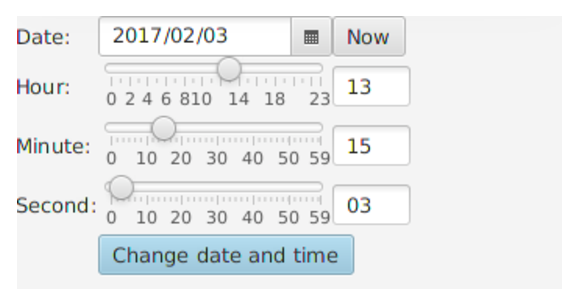
\includegraphics[scale=0.75]{setclock.eps}
	\caption{Setting the clock of the system}
\end{figure}

\begin{figure}[h]
    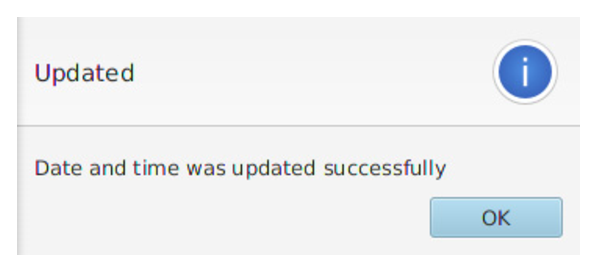
\includegraphics[scale=0.75]{setclock2.eps}
	\caption{Date and time was updated successfuly}
\end{figure}

\section{Login}
\label{operation:Login}

The user enters the system by entering credentials - login and password. The
user has three attemps to enter correct login and password, after three
unsuccessful attempts there is a captcha test. The user has to pass the captcha
test to make a new attempt of authentication.

\begin{description}
	\item \textbf{Parameters:} Login and Password
	\item \textbf{Precondition:} The system is started and the actor is not logged
	in. 
	\item \textbf{Post-condition:} If login and password are correct then the
	actor is logged in the system, otherwise - there is a notification
	of incorrect data and all the administrators are notified of an intrusion
	temptative. After getting incorrect credentials three times in a row the
	system causes a captcha test. 
	\item \textbf{Output messages:} ieMessage: "You are logged in! Welcome
	\ldots"
	
	\item \textbf{Triggering:}
	
	\begin{enumerate}
		\item In the iCrash authentification panel enter login and password, given by
		the supplier/administrator.
		\item Click on the button "Log on"
		\item In case of failure there is a notification of incorrect data.
		\item After three unsuccessful atempts the user has to pass the captcha test
		to try to login one more time.
	\end{enumerate}
\end{description}


\subsection{Login - example}

\begin{figure}[h]
    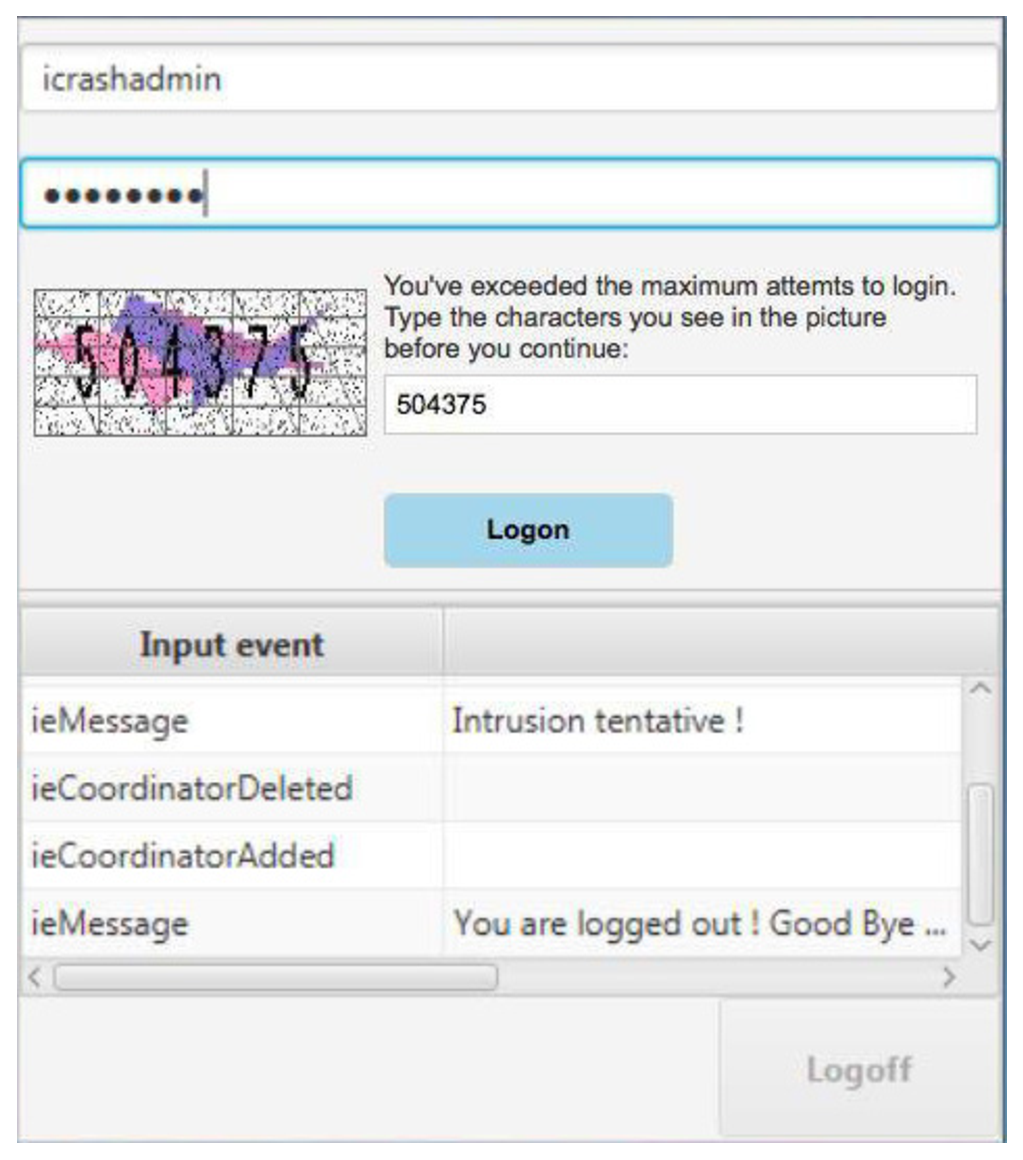
\includegraphics[scale=0.5]{login.eps}
	\caption{Captcha test}
\end{figure}



\section{Logout}
\label{operation:Logout}

The actor loggs out from the system.

\begin{description}
	\item \textbf{Parameters:} None
	\item \textbf{Precondition:} The system is started and the actor is logged in.
	\item \textbf{Post-condition:} The actor is logged out from the system.
	\item \textbf{Output messages:} ieMessage: "You are logged out! Good Bye
	\ldots"
	
	\item \textbf{Triggering:}
	
	\begin{enumerate}
		\item Click on the button "Log off"
	\end{enumerate}
\end{description}



\section{AddCoordinator}
\label{operation:AddCoordinator}

The administrator creates a new coordinator in the system.

\begin{description}
	\item \textbf{Parameters:} CoordinatorID, Login and Password
	\item \textbf{Precondition:} The system is started and the administator is
	logged in. CoordinatorID is a Integer greater than zero and lower or equal to
	5. Length of the Login value is not more than 20 characters. The length of the
	Password is at least 6 characters long.
	\item \textbf{Post-condition:} A new coordinator has been added to the system.
	\item \textbf{Output messages:} "ieCoordinatorAdded"
	
	\item \textbf{Triggering:}
	
	\begin{enumerate}
		\item Click on the button "Add a coordinator' and fill out the entries related
		to the personal information of a coordinator: CoordinatorID, Login and Password.
		\item Click on the button "Create".
	\end{enumerate}
\end{description}

\subsection{AddCoordinator - example}

\begin{figure}
    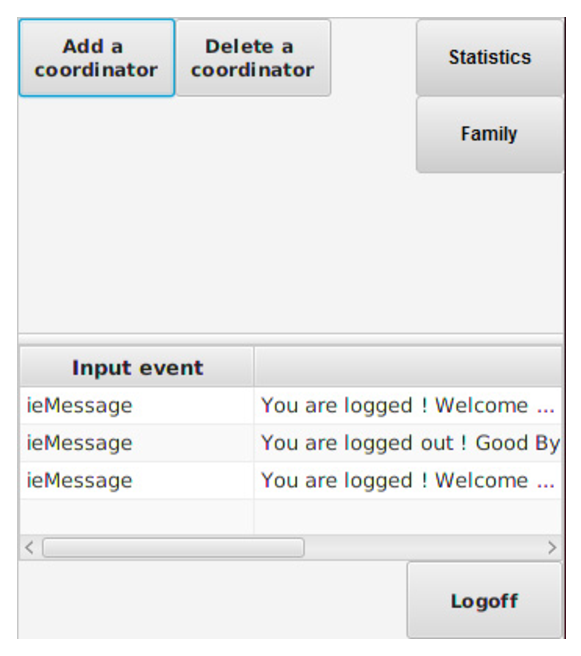
\includegraphics[scale=0.75]{admin.eps}
	\caption{Admins' panel}
\end{figure}

\begin{figure}
    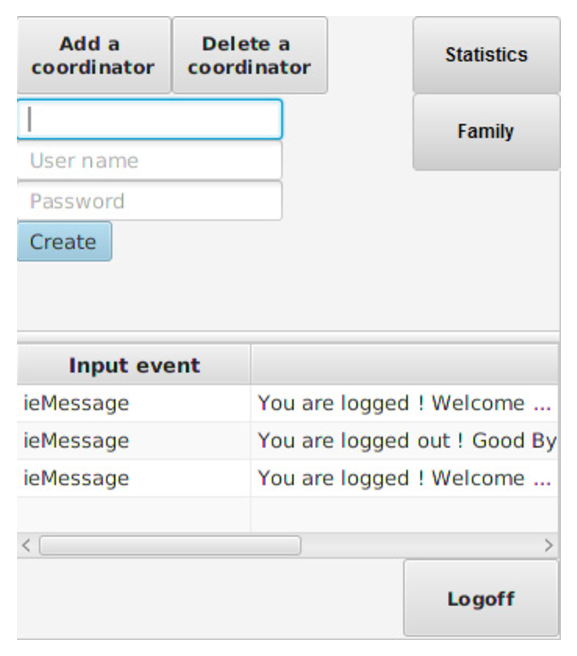
\includegraphics[scale=0.75]{addcoord.eps}
	\caption{Adding a coordinator}
\end{figure}



\section{DeleteCoordinator}
\label{operation:DeleteCoordinator}

The administrator deletes a coordinator from the system.

\begin{description}
	\item \textbf{Parameters:} CoordinatorID
	\item \textbf{Precondition:} The administator is logged in.
	\item \textbf{Post-condition:} The coordinator has been deleted from the
	system.
	\item \textbf{Output messages:} "ieCoordinatorDeleted"
	
	\item \textbf{Triggering:}
	
	\begin{enumerate}
		\item Click on the button "Delete a coordinator' and fill in the ID of the
		coordinator whom to delete.
		\item Click on the button "Delete". %%%% TODO: check the button whether it
		% is "Delete"
	\end{enumerate}
\end{description}


\section{HandleAlert}
\label{operation:HandleAlert}

An coordinator handles alerts received by changing their status.

\begin{description}
	\item \textbf{Parameters:} AlertID 
	\item \textbf{Precondition:} The system is started and the coordinator is
	logged in. 
	\item \textbf{Post-condition:} The status of the alert has been changed.
	\item \textbf{Output messages:} ieMessage: "The Alert is now declared as valid
	(or invalid)!"
	
	\item \textbf{Triggering:}
	
	\begin{enumerate}
		\item Choose an alert from the list and change its status by clicking on the
		button "Validate" or "Invalidate"
	\end{enumerate}
\end{description}

\subsection{HandleAlert - example}

\begin{figure}
    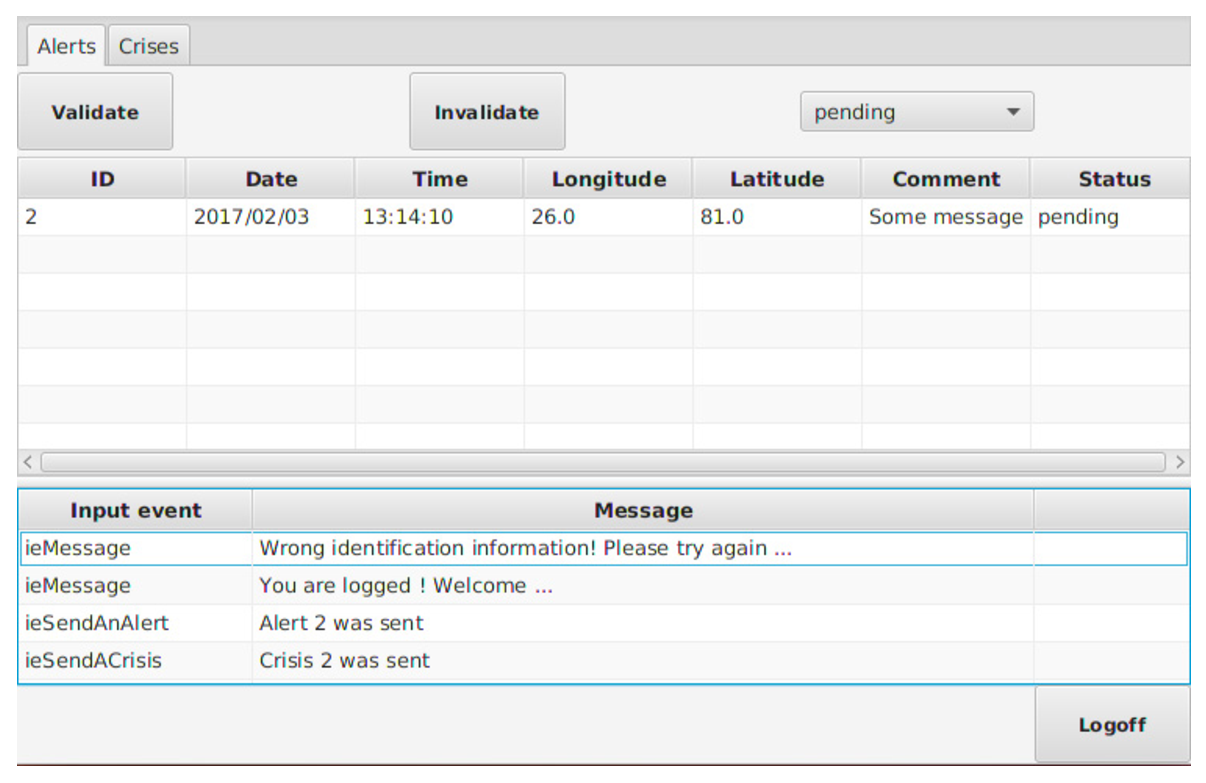
\includegraphics[scale=0.75]{handle_alert.eps}
	\caption{Coordinator panel - alerts}
\end{figure}




\section{GetAlertSet}
\label{operation:GetAlertSet}

An coordinator gets a set of alerts with particular status.

\begin{description}
	\item \textbf{Parameters:} AlertStatus 
	\item \textbf{Precondition:} The system is started and the coordinator is
	logged in.
	\item \textbf{Post-condition:} The list of alerts contains only alerts with chosen status.
	\item \textbf{Output messages:} None
		
	\item \textbf{Triggering:}
	
	\begin{enumerate}
		\item Choose a particular status from the drop-down list.
	\end{enumerate}
\end{description}



\section{GetCrisisSet}
\label{operation:GetCrisisSet}

An coordinator gets a set of crises with particular status.

\begin{description}
	\item \textbf{Parameters:} AlertStatus  
	\item \textbf{Precondition:} The system is started and the coordinator is
	logged in.
	\item \textbf{Post-condition:} The list of crises contains only crises with
	chosen status.
	\item \textbf{Output messages:} None
	
	\item \textbf{Triggering:}
	
	\begin{enumerate}
		\item Choose a particular crisis' status from the drop-down list.
	\end{enumerate}
\end{description}



\section{Alert}
\label{operation:Alert}

An operator of communication company sends an alert received from a human.

\begin{description}
	\item \textbf{Parameters:} HumanKind, Data, Time, PhoneNumber, GPSLocation,
	Comment
	\item \textbf{Precondition:} The system is initialized. Time of the alert is
	earlier than the current time of the system. The value of the latitude part
	of the GPSLocation is a real in the interval [-90.0 , +90.0]. The value of the longitude part
	of the GPSLocation is a	real in the interval [-180.0 , +180.0]. The length of
	the PhoneNumber is from 4 to 30 characters. The length of the Comment is
	not more than 160 characters.
	\item \textbf{Post-condition:} There is an alert with the status - "pending" in
	the list of alerts in coordinator panel. If there were no alerts before with the
	near location to the received alert there is a crisis with
	the same ID as the received alert has, the type - small, the status - pending.
	Else the received alert will be related to the nearest crisis initialized. 
	\item \textbf{Output messages:} None
	
	\item \textbf{Triggering:}
	
	\begin{enumerate}
		\item Choose a type of a person.
		\item Choose a date.
		\item Fill out the entries with the phonenumber, the latitude, the longitude
		and the comment.
		\item Set the time of the alert using scrollbars.
		\item Press on the button "Send alert" or in case of cancel - "Reset form".
	\end{enumerate}
\end{description}

\subsection{Alert - example}

\begin{figure}
    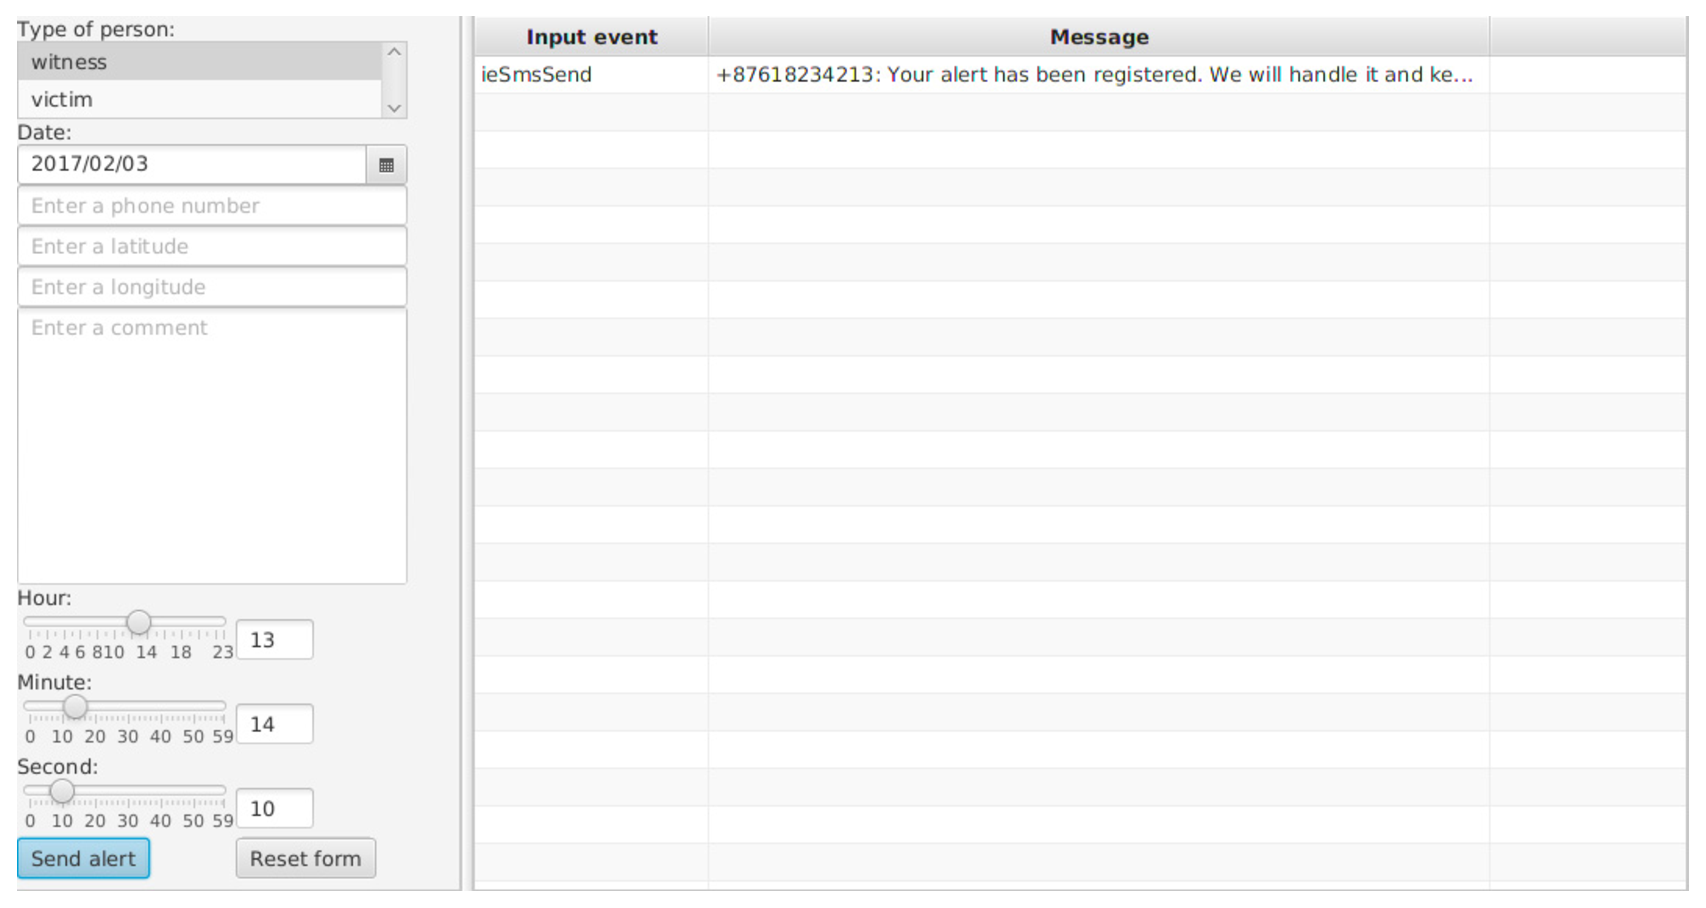
\includegraphics[scale=0.6]{com_company.eps}
	\caption{Communication company panel}
\end{figure}


\section{HandleCrisis}
\label{operation:HandleCrisis}

An coordinator handles a crisis by declaring himself as a handler of the crisis.

\begin{description}
	\item \textbf{Parameters:} CrisisID 
	\item \textbf{Precondition:} The system is started and the coordinator is
	logged in.
	\item \textbf{Post-condition:} The status of the alert has been changed to
	"handled". The crisis is associated to the coordinator who has handled the crisis.
	All the related alerts are sent to the coordinator. If the crisis was already
	handled its handler is updated to the new one and the previous handler is
	notified. A message to the related human is sent through the communication
	company.
	\item \textbf{Output messages:} ieMessage: "You are now considered as handling
	the crisis".
	
	\item \textbf{Triggering:}
	
	\begin{enumerate}
		\item Choose an alert from the list and press on the button "Handle crisis".
	\end{enumerate}
\end{description}

\subsection{HandleCrisis - example}

\begin{figure}
    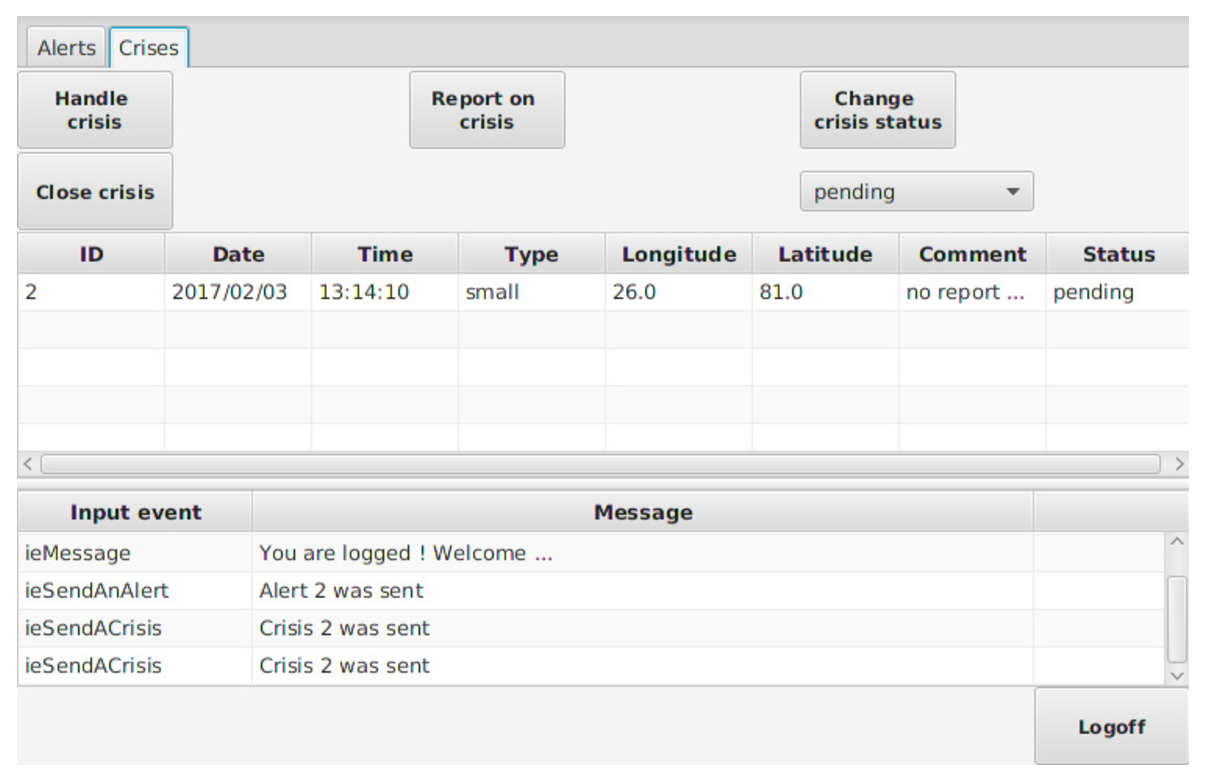
\includegraphics[scale=0.6]{crisis.eps}
	\caption{Coordinator panel - crises}
\end{figure}

\section{ReportOnCrisis}
\label{operation:ReportOnCrisis}

An coordinator updates the textual information for a crisis.

\begin{description}
	\item \textbf{Parameters:} CrisisID and Comment
	\item \textbf{Precondition:} The system is started and the coordinator is
	logged in. The length of the comment value is not more than 160 characters.
	\item \textbf{Post-condition:} The comment attribute of the crisis has been
	updated.
	\item \textbf{Output messages:} ieMessage: "The crisis comment has
	been updated "'
	
	\item \textbf{Triggering:}
	
	\begin{enumerate}
		\item Choose an alert from the list and press on the button "Report on crisis".
		\item Enter in the text field a report and press on the button "Report" or in case of cancel - "Cancel"
	\end{enumerate}
\end{description}


\section{SetStatusCrisis}
\label{operation:SetStatusCrisis}

An coordinator sets the status of a crisis.

\begin{description}
	\item \textbf{Parameters:} CrisisID and CrisisStatus
	\item \textbf{Precondition:} The system is started and the coordinator is
	logged in.
	\item \textbf{Post-condition:} The status of the alert has been changed.
	\item \textbf{Output messages:} ieMessage: "The crisis status has been updated !".
	
	\item \textbf{Triggering:}
	
	\begin{enumerate}
		\item Choose an alert from the list and press on the button "Change crisis
		status".
		\item Choose the status from the drop-box and press on the button "Change
		crisis" or in case of cancel - "Cancel"
	\end{enumerate}
\end{description}


\section{CloseCrisis}
\label{operation:CloseCrisis}

An coordinator closes a crisis.

\begin{description}
	\item \textbf{Parameters:} CrisisID
	\item \textbf{Precondition:} The system is started and the coordinator is
	logged in.
	\item \textbf{Post-condition:} The status of the alert has been changed to
	"closed". There is no handler associated to the closed crisis.
	\item \textbf{Output messages:} ieMessage: "The crisis is now closed !".
	
	\item \textbf{Triggering:}
	
	\begin{enumerate}
		\item Choose an alert from the list and press on the button "Close crisis".
	\end{enumerate}
\end{description}

\section{GetTimeStatistics}
\label{operation:GetTimeStatistics}

The administrator gets the list of alerts and crises on the concrete date or
within a defined period with extra time statistics.
When the alert was validated/invalidated; when the crisis was handled; all the times when the status was changed; when reported; when closed.
Also the administrator gets an average time for validating alerts and closing crises.


\begin{description}
	\item \textbf{Parameters:} Date/Period
	\item \textbf{Precondition:} The system is started and the administrator is
	logged in.
	\item \textbf{Post-condition:} There is the list of alerts/crises with all the
	time statistics.
	\item \textbf{Output messages:} None
	
	\item \textbf{Triggering:}
	
	\begin{enumerate}
		\item In the admin panel press on the button "Statistics".
		\item Press on the button "Alerts" or "Crises".
		\item Choose the date or press on the radio button "Period of time" for
		chossing a period.
		\item To get statistics - prress on the button "Get statistics".
		\item To close the statistics panel - press on the button "Close".
	\end{enumerate}
\end{description}

\subsection{GetTimeStatistics - example}

\begin{figure}[h]
    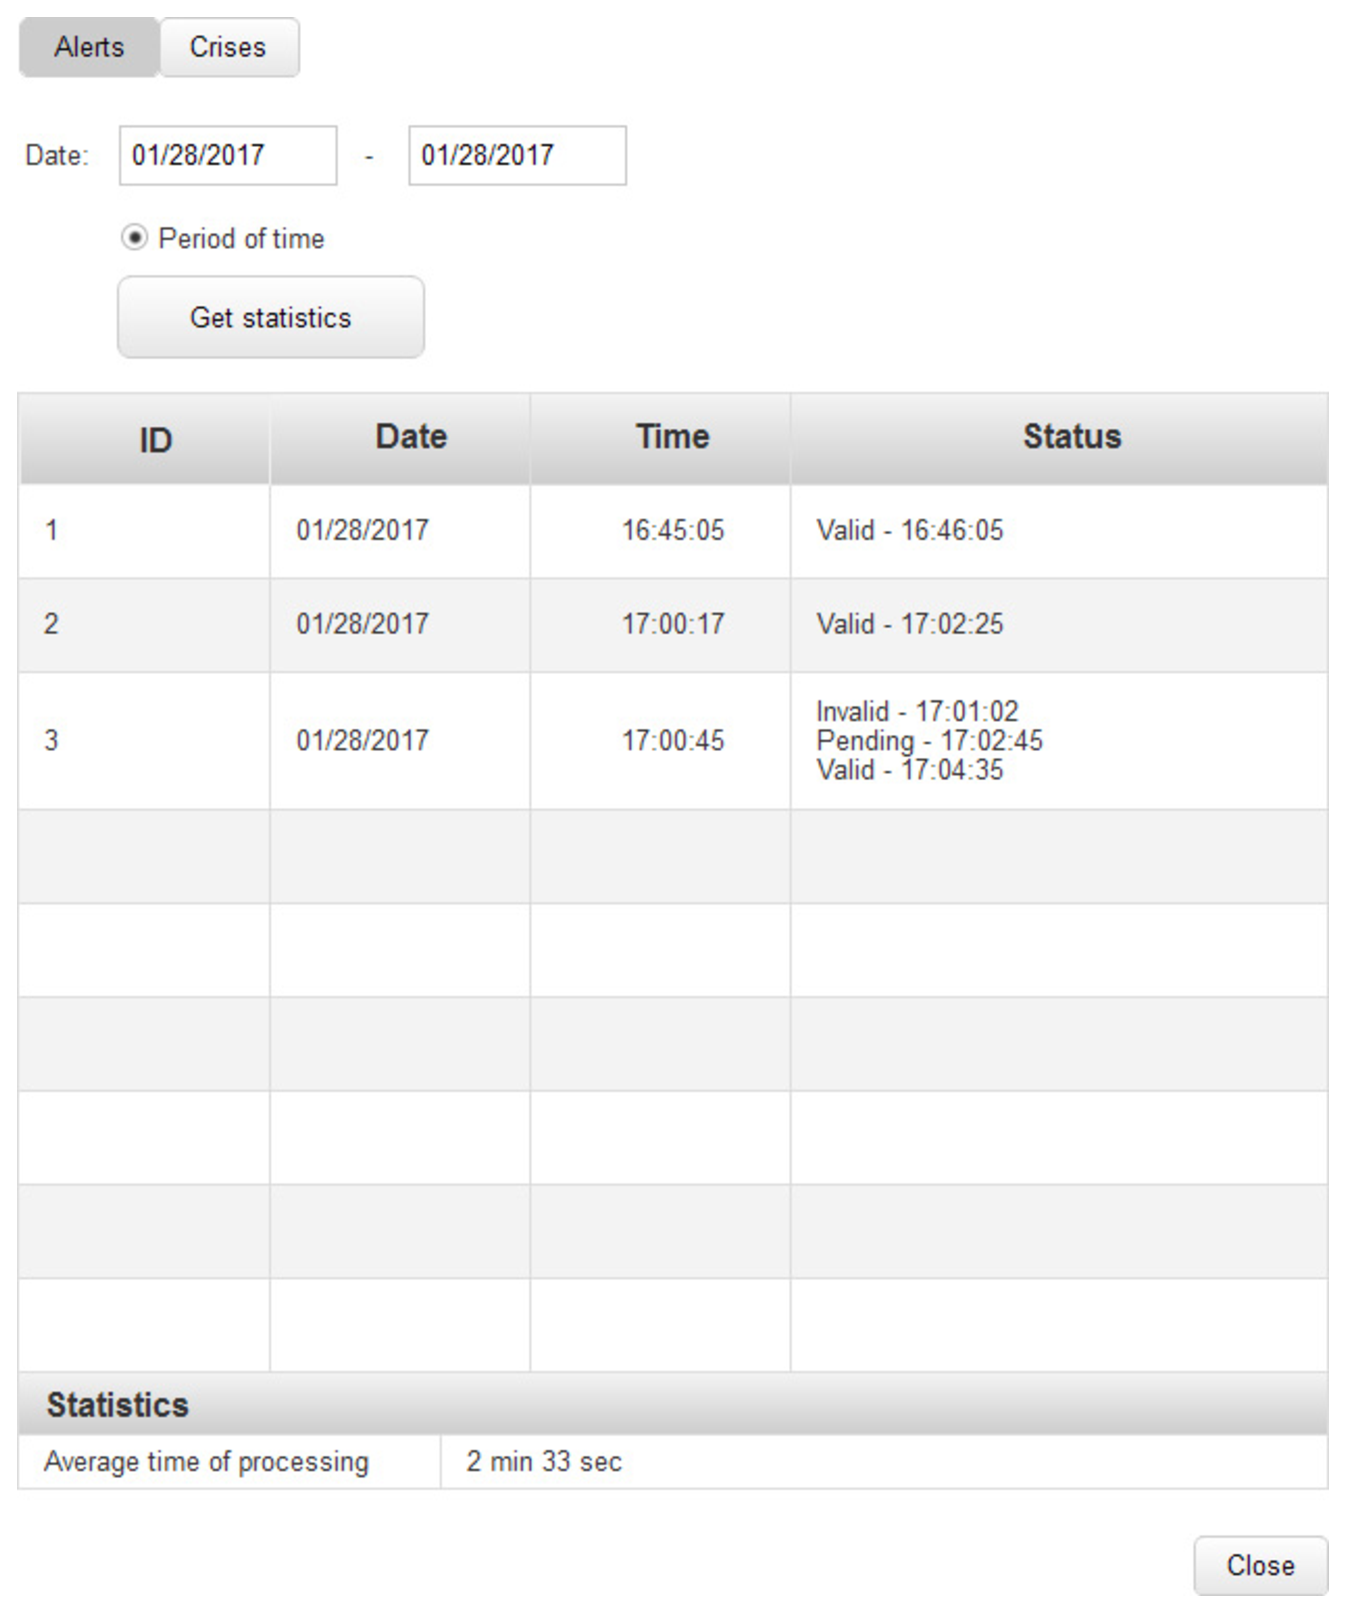
\includegraphics[scale=0.5]{alert_stats.eps}
	\caption{Time statistics of alerts}
\end{figure}

\begin{figure}[h]
    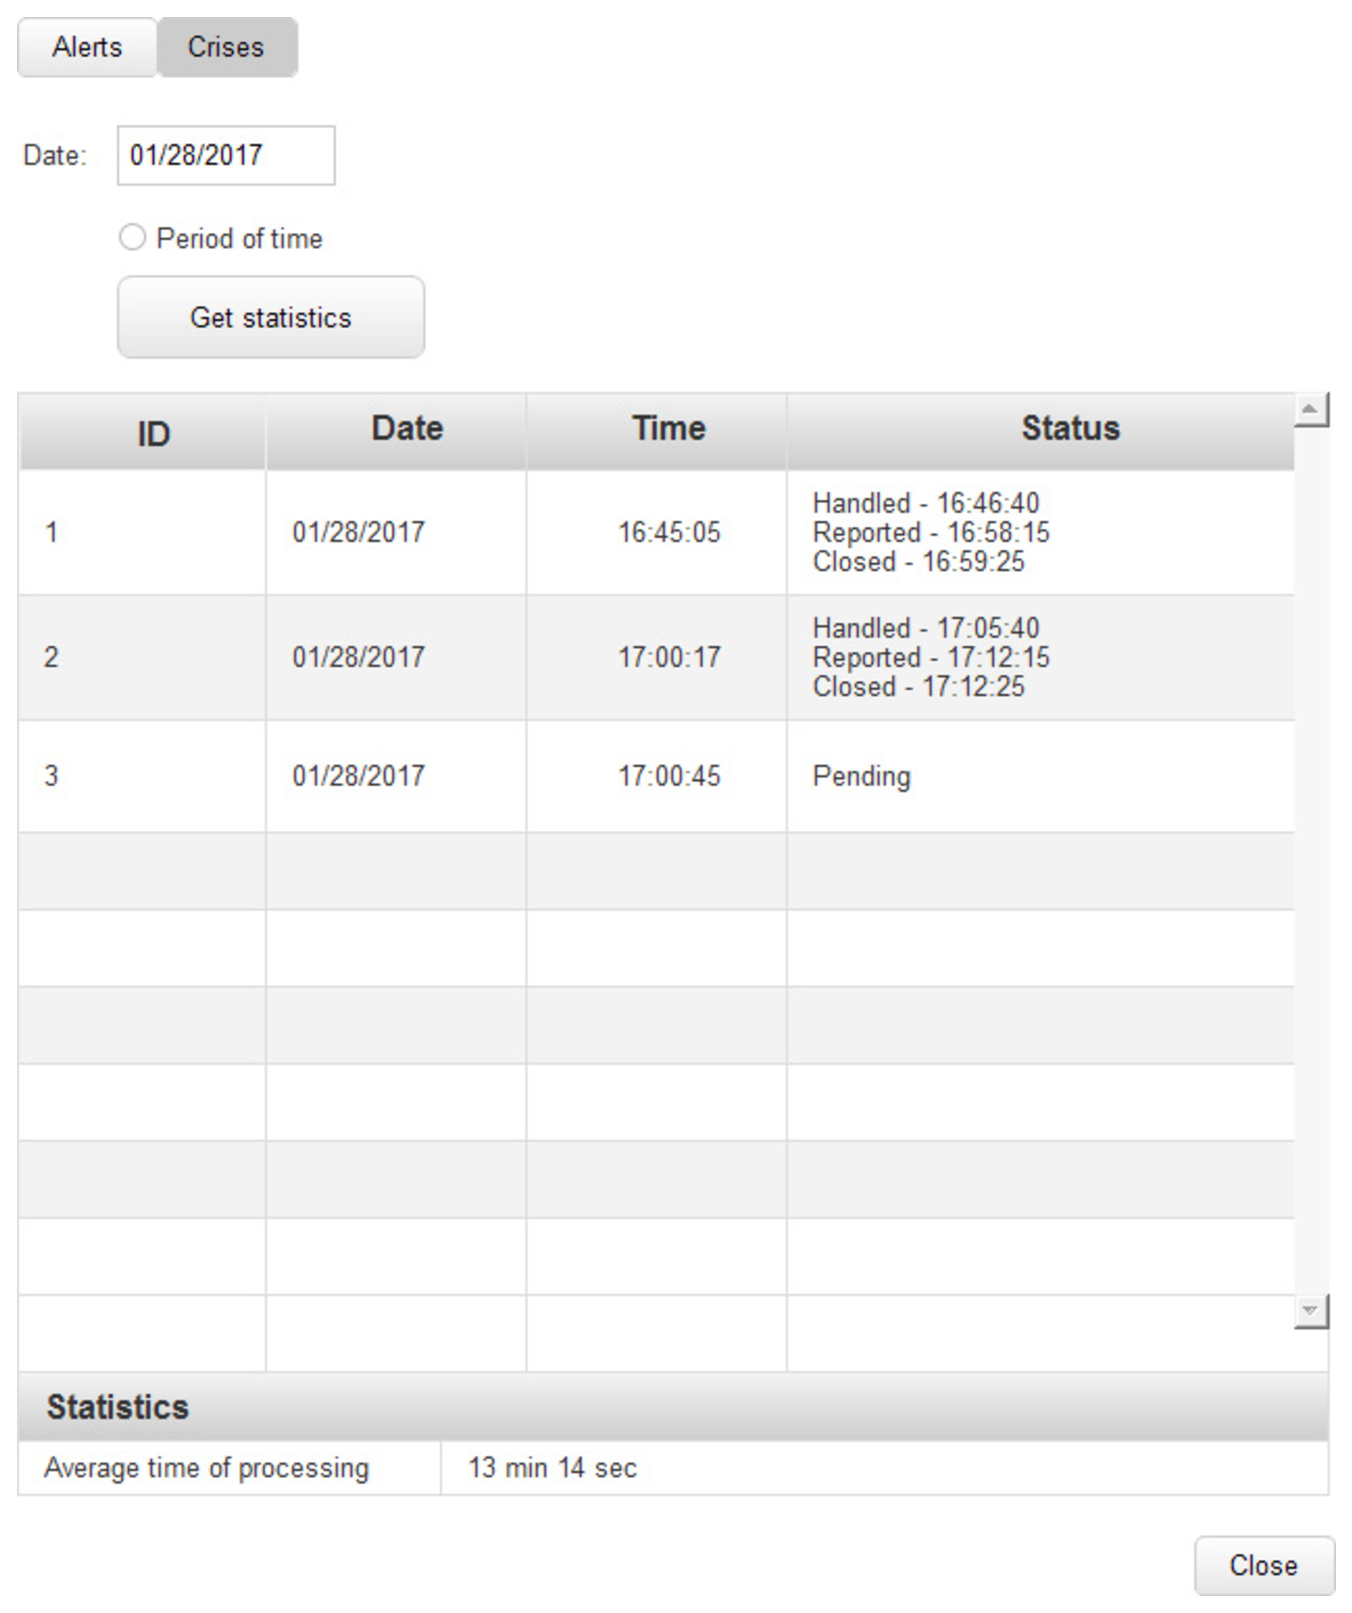
\includegraphics[scale=0.5]{crisis_stats.eps}
	\caption{Time statistics of crises}
\end{figure}




\newpage

% Error messages and problem resolution

\chapter{Error messages and problem resolutions}
\label{chap:error_messages}

\section{Error message 1}

\subsection{Problem identification}
When I try to log in through the iCrash admin system, it doesn't accept that
which is written in the readme file.

\subsection{Corrective actions}
1. The simplest way to know if all the VM are up and running is looking at the
messages that appear after you type vagrant up \\
2. Other thing you could try is to type in your console: vagrant box list .It
shows the different vagrant boxes already downloaded in your machine.\\
3. Also in case of using Vagrant project you need to check if all virtual
machines were started correctly. In particular you should login into the server VM and see if the server has been started: you can do it by typing:  ps -ax | grep java which displays all Java processes running on the machine.



\section{Error message 2}

\subsection{Problem identification}
I made iCrash project changes in order to implement the variants. Before
changing I could start the project but after modifications, an error is
displayed. I think maybe this is an error in the server.\\
\begin{center}
\includegraphics[width=0.5\textwidth]{./images/er1.eps}
\end{center}

\subsection{Probable cause}
This problem may happen because you made a copy of the iCrash project into the
same workspace (let's say you decided to called iCrash2), but you did not change
the Web Project settings configuration\\

\subsection{Corrective actions}
Right-click on the project->properties, then select Web Project Settings. You
need to change the context root to a name other than iCrash (maybe iCrash2).\\
In case you still have problems to run the web application, have a look into the file server.xml, placed inside the Servers project, into the folder Tomcat v8.0 Server. Search for the entries "Context" and ensure that the property path points to the right context for each entry appearing into the file.
 

\section{Error message 3}

\subsection{Problem identification}
I would like to modify a class in iCrash H5, whose GUI was created with Vaadin
Designer, but it looks broken and is unmodifiable. What could I do?\\
\begin{center}
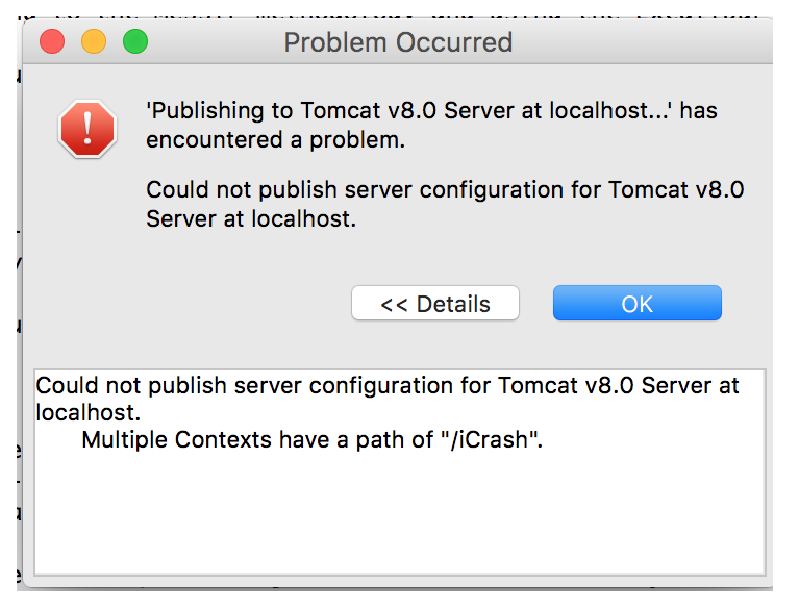
\includegraphics[width=0.5\textwidth]{./images/er2.eps}
\end{center}

\subsection{Probable cause}
GUI might not be supported by your drivers.
 
\subsection{Corrective actions}
Method 1: 
You need to change ComCompanyDesign's theme from icrash to valo.
It then solves the problem:
\begin{center}
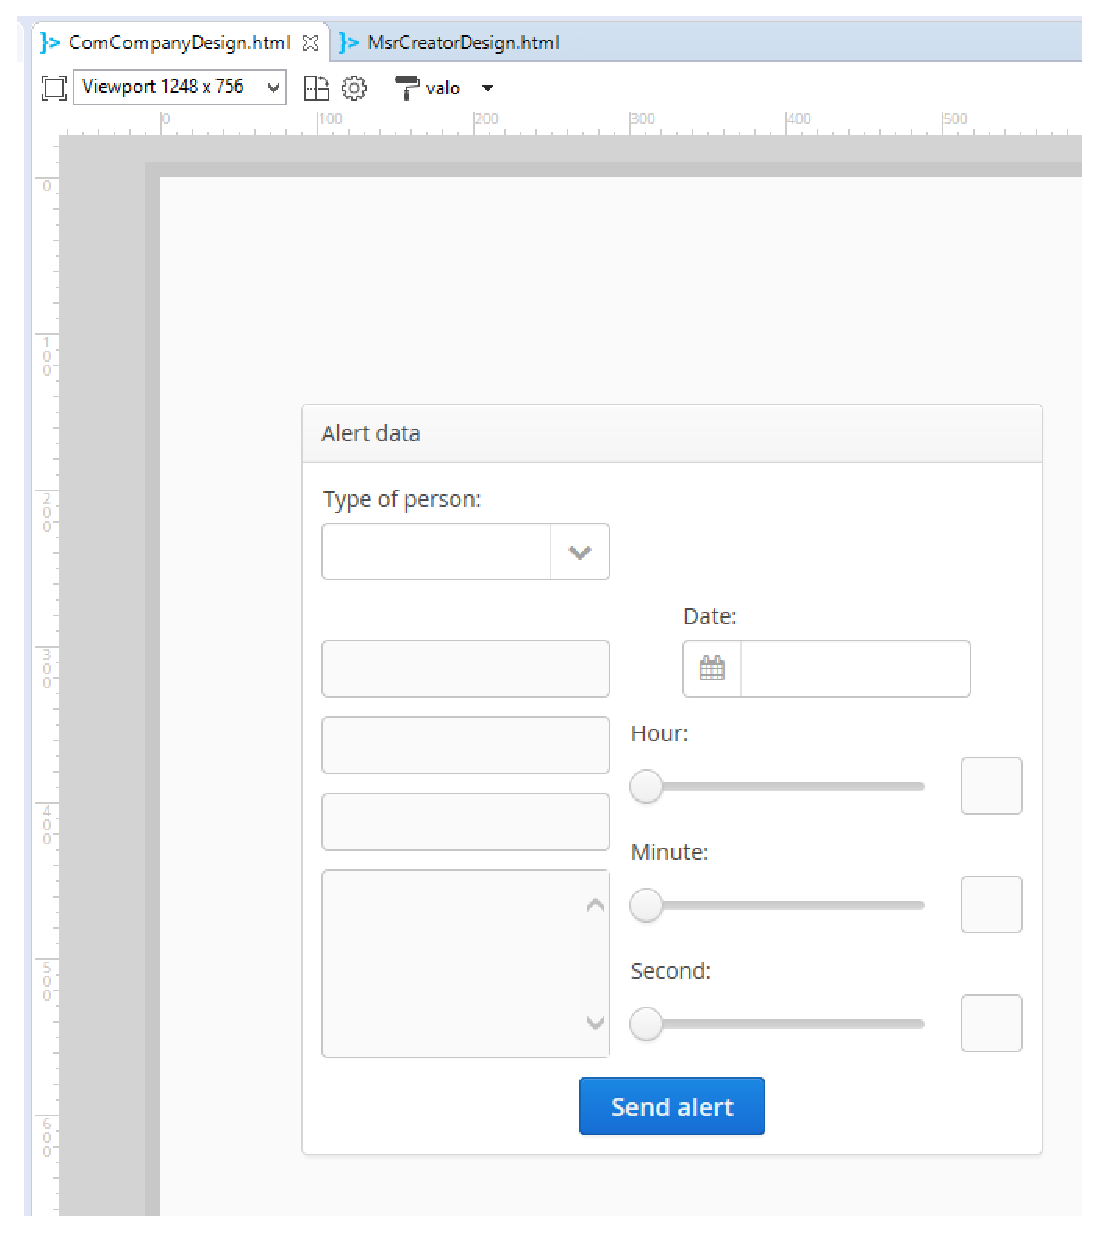
\includegraphics[width=0.5\textwidth]{./images/er3.eps}
\end{center}

Method 2:\\
Unzip 1.zip to project's WebContent VAADIN-themes-icrash\\
Clean the project (build automatically should be on) and reopen ComCompanyDesign.
You will then get the same result with icrash theme - the design will become editable.


\section{Error message 4}

\subsection{Problem identification}
When compiling a message indicates that there is a file missing.

\subsection{Probable cause}
Issues with correct PATH.

\subsection{Corrective actions}
You need to ensure that:\\
1) you are using Excalibur v1.5.1\\
2) you have the latest version of the Excalibur Standard Libraries setup in your
environment, If not sure, then remove the projects from the workspace, and then
add them again.\\ 3) you have the latest released iCrash Specification in your
workspace. If not sure, then remove the project from the workspace and add it
again. \\
Once you have ensured the previous steps, check if the problem remains.


\section{Error message 5}

\subsection{Problem identification}
Is it normal that all the views (even the ones that come with the icrash
specification project) and their documentation are missing? Is there a way to recover the views that come with the project and their captions?

\subsection{Probable cause}
Problems with displaying data.

\subsection{Corrective actions}
No it is normal that all the original views of the icrash specification project
are missing and their documentation are missing.\\
1. Close Eclipse\\
2. You can copy/paste the following files from the original icrash project to
your icrash variant project.\\
2.a the representation.aird file\\
2.b all msrd files in the folder lu.uni.lassy.excalibur.examples.icrash/views"\\
3 Launch Eclipse\\


\newpage

%APPENDICES
\appendix
% Last Modification:
% @author AUTHOR_NAME
% @date TODAY_DATE



\newpage

   
%GLOSSARY
%Uncomment the line below if you want to print all glossaries no matter if they
% appear in the document
%\glsaddall
\printglossaries
\newpage

 
%BIBLIOGRAPHY
\cleardoublepage 
\bibliographystyle{./../lu.uni.lassy.excalibur.standard.report.libraries/styles/lncs} 
\bibliography{./../lu.uni.lassy.excalibur.standard.report.libraries/defs/references/messir,doc/bibliography/user-manual}
\label{sec:references}

 
\end{document}
